%\documentclass[twoside,openright,a4paper,12pt,english,draft]{article}
\documentclass[twoside,openright,a4paper,12pt,english]{article}

%\documentclass[twoside,openright,a4paper,11pt,french]{article}
%\documentclass[twoside,openright,a4paper,11pt,french]{book}
\usepackage[utf8]{inputenc}
\usepackage[english]{babel}

% Utilisation de tableaux
\usepackage{tabularx}
\usepackage{listings}             % Include the listings-package
 \lstset{language=Java}          % Set your language (you can change the language for each code-block optionally)

\usepackage{subcaption}
\usepackage{wrapfig}

% Utilisation d'url
\usepackage{url}
\urlstyle{sf}

% Utilisation d'images, stockées dans le répertoire ./pics/
\usepackage{graphicx}
\graphicspath{pics/}

% Définition des marges
\usepackage{geometry}
\geometry{%
  left=30mm,%
  right=30mm,%
  top=35mm,%
  bottom=45mm,%
  foot=15mm% 
}

\begin{document}

%%% IRBABOON
\def\j{\emph{Jitsi}}
\def\jvb{\emph{Jitsi Videobridge}}
\def\bj{\emph{BlueJimp}}
\def\lj{\emph{libjitsi}}
\def\wrtc{\emph{webrtc.org}}
\def\jm{\emph{Jitsi Meet}}


%%% NOOBABRI

% La page de garde
\thispagestyle{empty}

\begin{center}
       \noindent
       
\includegraphics[height=2.5cm]{./pics/uds.eps}       
       
       \vfill\vfill

    {\large \textsc{Master 2\\Réseaux Informatiques et Systèmes Embarqués}}

    \bigskip\bigskip

    {\large Presented by}
    %{\large Présenté par}

    \medskip

% Identité de l'auteur
    {\large Boris \textsc{Grozev}}
 
% Contact mail ou téléphone   
    {\small \url{boris@jitsi.org}}

    \vfill\vfill

% Titre du stage
    {\huge \sc
      \begin{center}
		Final Report
      \end{center}}
        \begin{center}
        Media recording for multiparty video conferences based on WebRTC %XXX discuss title
        \end{center}

    \vfill\vfill

    {\large Supervised by:}

\medskip

% Identité de l'encadrant
    {\large Emil \textsc{Ivov}}

% Contact mail ou téléphone
    {\small \url{emcho@jitsi.org}}

\bigskip

    {\large Hosting enterprise:} %XXX that sounds terrible
    %{\large Au sein de}

\medskip

% Structure d'accueil
    {\large \textsc{BlueJimp}}

\vfill\vfill\vfill
           
% Logo de votre structure d'accueil
       %
\includegraphics{./pics/bluejimp2.eps}       
       
\includegraphics[height=2.5cm]{./pics/bluejimp2.eps}

\end{center}


% Page blanche au dos de la page de garde
\newpage
\pagestyle{empty}
\newpage


% La table des matières
\parskip=0pt
\tableofcontents

% Page blanche entre la table des matières et le texte
\newpage
\pagestyle{empty}
\newpage

\pagenumbering{arabic}
\thispagestyle{plain}
\pagestyle{plain}


\begin{abstract}
This document describes the implementation of various media recording-related
features in a modern video conferencing application based on WebRTC. We start
by introducing the work environment and the various technological components
involved in the project. We then proceed with a detailed description of the
different stages of the project including the way audio and video data is
transported over the network, the way it is persistently stored, synchronized,
and the way multiple audio and video files are organized and combined in a
single flat audio/video file. The work on the project is still actively
pursued and we therefore also present a number of planned future steps and
improvements that will likely be implemented in the near
future.

%This document describes work done
%during a 6-months long internship. It describes a modern video
%conferencing application based on WebRTC (\jm) discussed, and a system for
%media recording, which I helped to design and implement, is examined in detail.
%The first section introduces the work environment for the
%internship and the most important relevant standards and technologies. The rest 
%of the sections examine specific parts of the media recording system.
\end{abstract}




\section{Introduction}
\label{chap:intro}
The ever decreasing cost of bandwidth and processing resources have in the recent years
made multi-party video conferencing over the internet viable for personal use. The advent of the WebRTC
technology that adds audio/video communication capabilities to web browsers,
has made the development of conferencing application (or the addition of
conferencing features to existing applications) simpler than ever before.

The work described in this document is about the development of video recording features
within \jm: an existing WebRTC video conferencing application. Through
the rest of this section we introduce the working environment, the most
important standards and software products used in \jm, and we discuss the
general concept of recording a conference. In sections \ref{recording-video} through \ref{dsd} we examine specific
parts of the recording process in detail. In section \ref{future-work} we
discuss new features and optimizations to existing features which we plan to
develop in the near future. In section \ref{conclusion} we review accomplished work.


XXX Problematique, objectifs

XXX mise en relation des besoins de l’entreprise et des objectifs des missions mise en perspective de ces missions : en quoi cela apporte qq chose cahier des charges

XXX mode de travail (avec qui ? qui fait quoi ?)

XXX planning
\subsection{\bj}
XXX expand?

\bj\footnote{\url{https://bluejimp.com}} is a small company which
offers support and development services mainly focused around the
\j\footnote{\url{https://jitsi.org}}
 family of projects. The FLOSS (Free/Libre Open Source Software)
nature of these projects makes for a slightly unusual business model. The
company works with various kinds of customers who all have different use cases
for \j\ and need it adapted to their needs. While \bj\ has no exclusivity
on such adaptations, it is tightly involved in the development of the project
and some of the related technologies and standards. This has helped the company
acquire significant credibility and offer advantageous price/quality ratios.

In addition to orders from customers, \bj\ also often works on internal projects
that aim to enrich \j\ and make it more attractive to both users and
enterprises. 

\bj\ is registered in Strasbourg, but the development team is international,
with people working from different geographic locations. Most communication happens over
the Internet using e-mail, instant messaging and audio/video calls.

My position in \bj\ is that of a software developer. Apart from development, my tasks also 
involve a fair amount of research, experimentation and optimizations. I have
worked on \j\ previously and when my internship began, I was able to quickly
get accustomed to the environment. 




\subsection{The \j\ family}
\label{intro-jitsi}

\j\ is a feature-rich internet communications client.
It is free software, licensed under the LGPL\cite{lgpl}.
The project was started by Emil Ivov in
the University of Strasbourg in 2003, and it was then known as SIP
Communicator. In the beginning
SIP Communicator was only a SIP client, but through the years it has evolved
into a multi-protocol
client (XMPP, AIM, Yahoo! and ICQ are now also supported) with a very wide variety
of features: instant messaging (IM), video calls, desktop streaming,
conferencing (multi-party, both audio and video), cross-protocol calls (SIP to
XMPP), media encryption (SRTP),
session establishment using ICE, file transfers and more.
Most of the development is financed by \bj.

\j\ is written mostly in Java and runs on a variety of
platforms (Windows, Linux, MacOSX and Android). The various projects comprise a massive codebase--
over 700 000 lines of Java code alone.

A big part of the code which was originally in \j\ is now split into a
separate library-- \emph{libjitsi}. This allows it to be easily reused in other
projects, such as \jvb. The code in \lj\ deals mainly with multimedia-- capture
and rendering, transcoding, encryption/decryption and transport over the
network of audio and video data. It contains the RTP stack for \j\ (partially
implemented in \lj\ itself, partially in the external FMJ library).

\jvb\ is a server-side application which acts as a media
relay and/or mixer. It allows a smart client to organize a conference
using an existing technology (for example, SIP or XMPP/Jingle), outsourcing the bandwidth-intensive task of media relaying to a server. 
The organizing client controls \jvb\ over XMPP\footnote{Although a REST API is also available.}, while the rest of the
participating clients need not be aware that \jvb\ is in use (for example they
can be simple SIP clients). Since the end of 2013 \jvb\ supports ICE and is WebRTC-compatible.

One of the latest additions to the \j\ family is
\jm\footnote{\url{https://jitsi.org/Projects/JitsiMeet}}. This is a WebRTC
application, which runs completely within a browser and creates a video
conference using a \jvb\ instance to relay the media.




\subsection{WebRTC}
WebRTC (Web Real-Time Communications) is a set of specifications 
currently in development, that allow browsers which implement them to open
"peer connections". These are direct connections between two
browsers (a webserver is used only to setup the connection), and can be used to
send audio, video or application data. The specifications are open and are meant
to be implemented in the browsers themselves (without the need for additional
plug-ins).

WebRTC is divided in two main parts: the JavaScript standard APIs, being defined within
the \emph{WebRTC} working group\cite{webrtc-wg} at W3C,
and the on-the-wire protocols, being defined within
the \emph{RTCWEB} working group\cite{rtcweb-wg} at the IETF.

These standards provide web developers with a very powerful tool, which
can be used to easily create rich real-time multimedia applications.
There is also the possibility to pass arbitrary data in an 
application-defined format. These allow for some very interesting and more
complicated use-cases. 

The specifications are still being developed, but are already at an advanced stage. There is
an open-source implementation of the network protocols, provided by Google with
a BSD-like license. I will refer to this implementation as \emph{webrtc.org}
(which is the domain name of the project). Currently all browsers implementing
WebRTC (Chrome/Chromium, Opera and Mozilla Firefox) 
use \emph{webrtc.org} as their base. Because of this, \wrtc\ is very important -- it is
used for all practical compatibility testing, making it the de-facto reference implementation.




\subsection{XMPP and Jingle}
Extensible Messaging and Presence Protocol (XMPP)\cite{rfc6120} is a mature,
XML-based protocol which allows endpoints
to exchange messages in near real-time. The core XMPP protocol only covers instant messaging (that is the exchange of
text messages meant to be read by humans), but there are a variety of extensions that allow the protocol
to cover a wide range of use cases. Many such extensions are published as XMPP Extension Protocols (XEPs), and there are XEPs for
group chats, user avatars, file transfers, account registration, transporting
XMPP over HTTP, discovery of node capabilities, management of  wireless sensors (provisioning, control, data collection),
and, most relevant here, internet telephony.

\emph{Jingle} (defined in XEP-0166\cite{jingle166} and XEP-0167\cite{jingle167})
is a signalling protocol, serving a purpose similar to that of SIP: it uses an
offer-answer model to setup an RTP session. Many of the
protocols often used with SIP, such as ICE\cite{ice}, ZRTP\cite{zrtp}, DTLS-SRTP\cite{rfc5763}, and
RFC4575\cite{rfc4575} can also be used with \emph{Jingle}. Mappings
have been defined between the two\cite{stoxmedia}, which allow gateways or rich
clients to organize cross-protocol calls.

\begin{wrapfigure}{r}{0.4\textwidth}
   \centering
        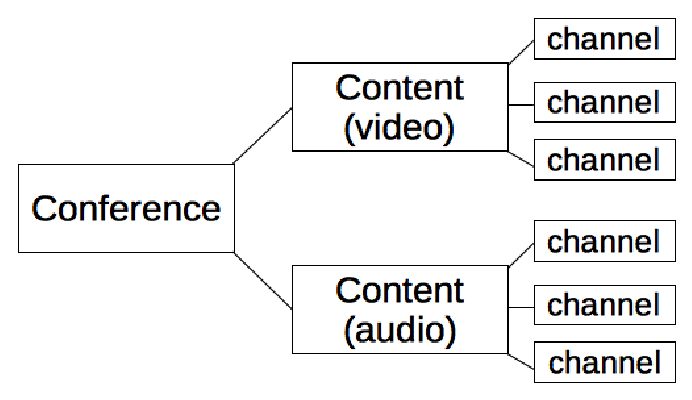
\includegraphics[width=0.35\textwidth]{./pics/colibri-conf.eps}
        \caption{A COLIBRI conference.}
   \label{colibri-conf}
\end{wrapfigure}

COnferencing with LIghtweight BRIdging (COLIBRI\cite{colibri}) is an extension
developed mostly in \bj\ for use with \jvb. It provides a way for a client to control a multimedia
relay or mixer, such as \jvb. It works with the concept of a \emph{conference}, which contains
\emph{channels}, separated in different \emph{contents} (see fig.\ref{colibri-conf}).
In the most common use case a client requests the creation of a \emph{conference} with a specified number of
channels. The mixer allocates local sockets for each \emph{channel} and
provides their addresses to the client. The client then uses these transport
addresses as its own to establish, for example, a \emph{Jingle} call. 
Instead of just allocating local sockets, the ICE protocol can be used, in
which case the mixer provides a list of ICE candidates for each \emph{channel}.
The protocol works with a natural XML representation of a \emph{conference}.
After the \emph{conference} is established, the client can add or remove channels
from it, or change the parameters (such as the direction in which
media is allowed to flow) of an existing \emph{channel}.





\subsection{\jm}
\label{intro-jm}
\jm\ uses the above-mentioned technologies to create a multi-party video conference.
The endpoints of the conference are simply WebRTC-enabled
browsers\footnote{Although at the present time only Chrome/Chromium and Opera are
supported.} running the actual \jm\ application. They all connect to an XMPP
server and join a Multi-User Chat (MUC) chatroom. One of the participants (the
first one to enter the chatroom) assumes the role of organizer (or focus).

The focus creates a COLIBRI conference on a \jvb\ instance (\emph{jvb}), and allocates
two COLIBRI channels for each participant (one for audio, and one for video).
Then, it initiates a separate \emph{Jingle} session with
each participant, using the
transport information (i. e. the list of ICE candidates) obtained from $jvb$
instead of its own. When the participants accept the Jingle sessions, they in
effect perform ICE and establish direct RTP sessions with $jvb$.

The resulting connections for signalling and media are depicted in Figures
\ref{jitmeet-sig} and \ref{jitmeet-med} respectively.


\begin{figure}[h]
   \centering
        \begin{subfigure}[t]{0.4\textwidth}
            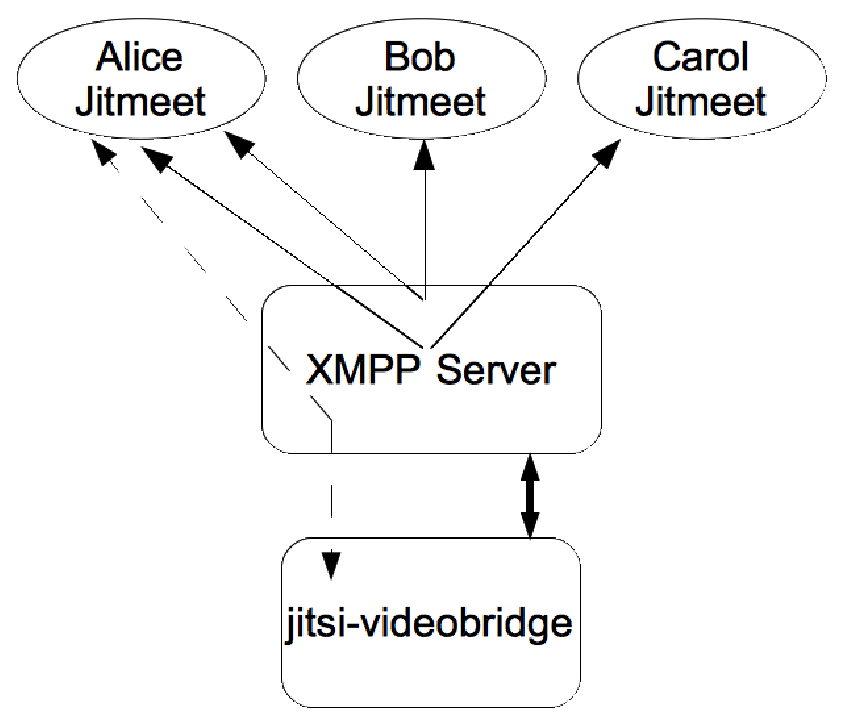
\includegraphics[height=5.5cm]{./pics/jm-sig.eps}
            \caption{Signalling connections in a \jm\ conference.
                The solid lines are XMPP/Jingle sessions, the dashed line
                is XMPP/COLIBRI. The thick line is an XMPP Component Connection.}
            \label{jitmeet-sig}
        \end{subfigure}
        \quad
        \quad
        \quad
        \begin{subfigure}[t]{0.4\textwidth}
            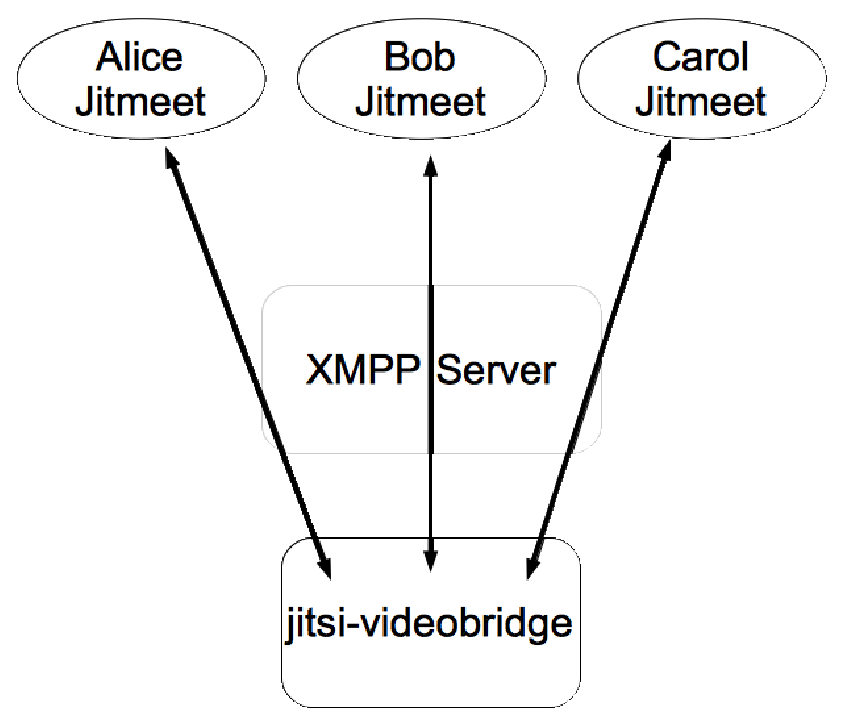
\includegraphics[height=5.5cm]{./pics/jm-med.eps}
            \caption{Media connections in a \jm\ conference. The
                lines represent RTP/RTCP sessions.}
            \label{jitmeet-med}
        \end{subfigure}
\end{figure}

The \jvb\ instance runs as a relay (as opposed to a mixer) for both video and
audio (meaning that it only passes RTP packets between the participants,
without considering their payload).

\smallskip
On the user-interface end, \jm\ aims to make it as easy as possible for a
person to enter or organize a conference. 
Entering a conference is accomplished by simply opening a URL such as \emph{https://meet.jit.si/ConferenceID} 
(where \emph{ConferenceID} can be chosen by the user). If \emph{ConferenceID}
doesn't exists, it is automatically created and
the user assumes the role of focus, inviting anyone who enters later on. If
\emph{ConferenceID} exists,
the user joins it (possibly after entering a password for the conference).

When in a conference, the interface has two main elements: one big video
(taking all available space) and, overlayed on top of it,
scaled down versions of the videos of all other participants. Figure
\ref{jm-ss} is a screenshot from the actual application. Current work is underway to
use dominant speaker identification (see section \ref{dsd}) to change the video
shown in full size to the person currently speaking.

\begin{figure}[h]
    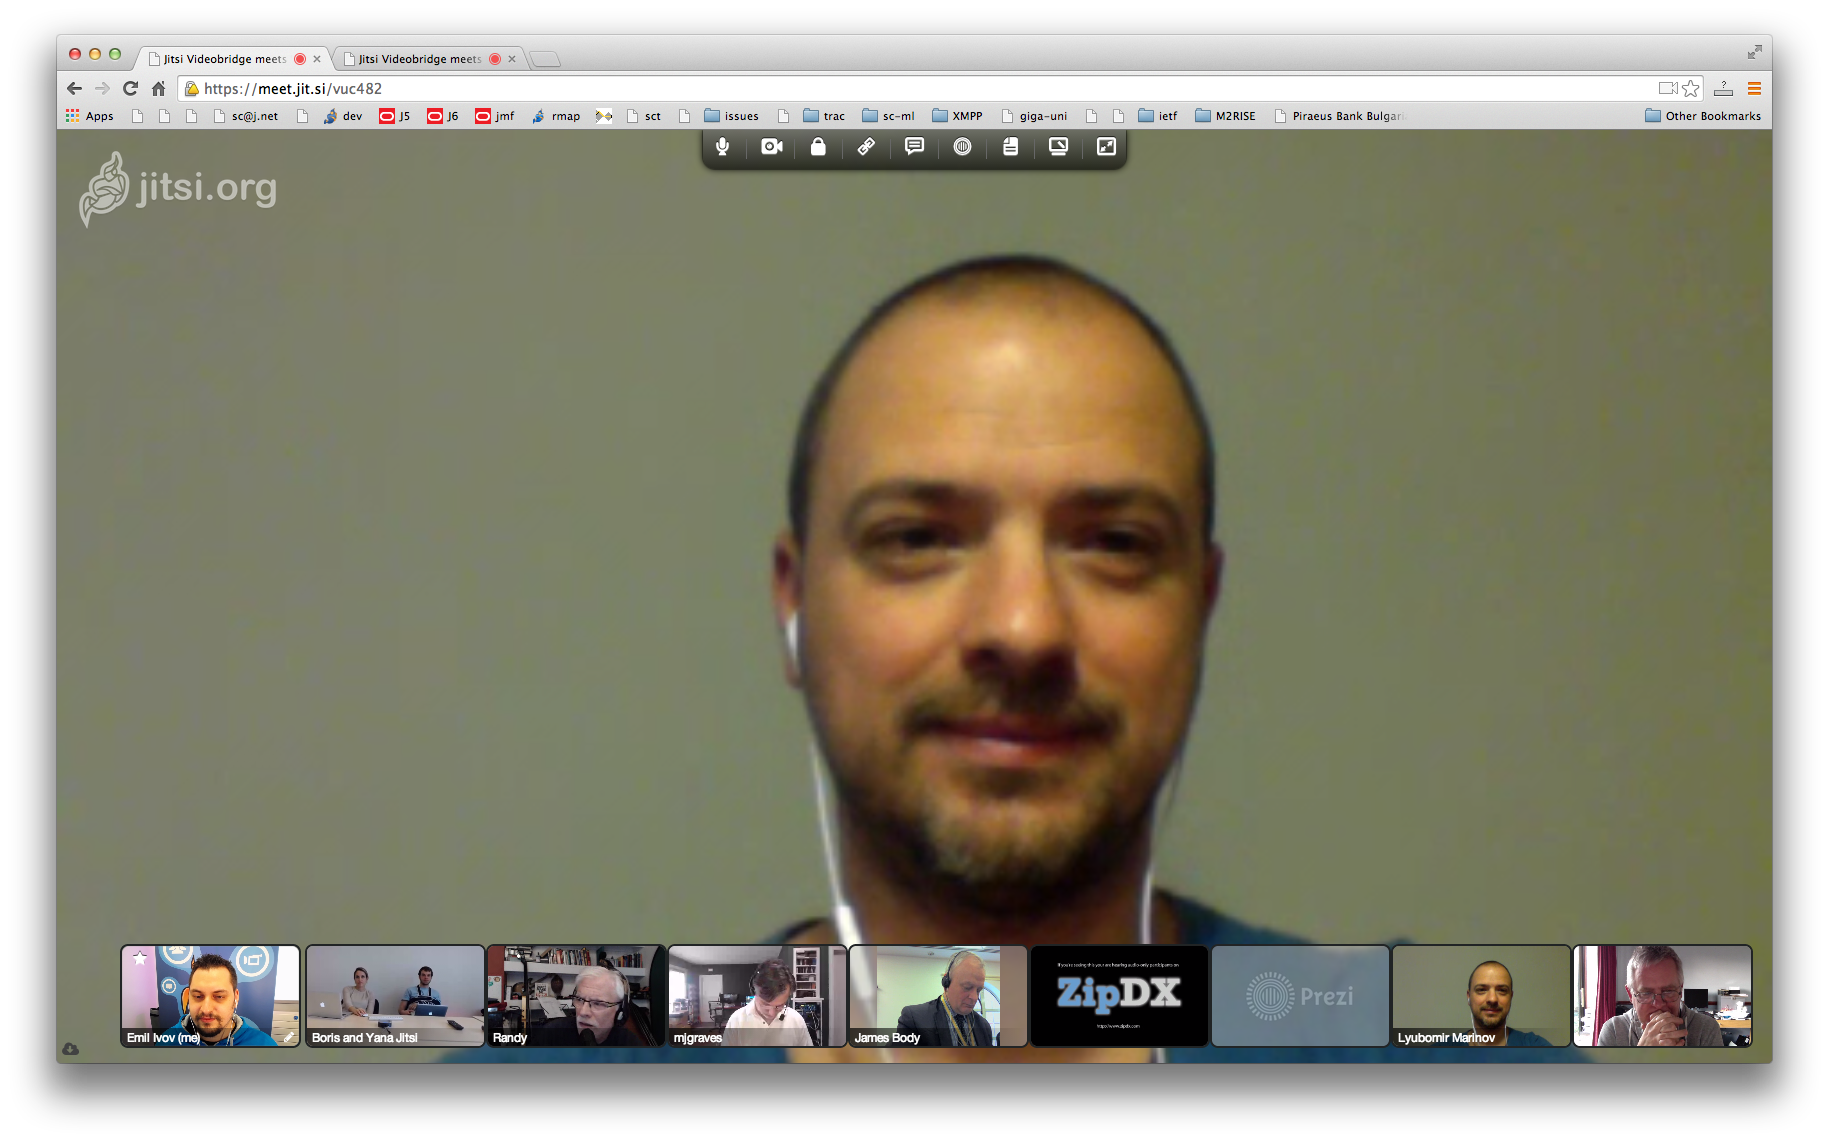
\includegraphics[width=1\textwidth]{./pics/jm-ss.eps}
    \caption{A screen capture from a \jm\ conference.}
    \label{jm-ss}
\end{figure}

\medskip
In contrast to other products for video conferencing over the internet, the
whole infrastructure needed to run \jm\ can be installed in a custom
environment. The only services which are needed are a web server
(only serving static content), an XMPP server, and an instance of \jvb. This
makes \jm\ very suitable for businesses (or even individuals) who want full
control over their conferencing solution.



\subsection{Recording}
\label{intro-recording}
By recording a multimedia conference in general we mean the following: all the
audio and video from the conference
is saved to disk in some format, in a way which allows the whole conference to
be played back later on.

\medskip
In our specific case, the recording of a conference has four main parts:
\begin{itemize}
\item{Recording video}
\item{Recording audio}
\item{Recording metadata}
\item{Post-processing}
\end{itemize}

Recording of the media is the process in which the audio and video RTP streams
in the conference are converted to a convenient format and saved to disk. There
are many different ways in which this can be done. Our final solution (and some
of the ideas that didn't work) are discussed in detail in
sections \ref{recording-video} and \ref{recording-audio}.

Recording of metadata means saving additional information (apart from the media
itself) which is necessary to play back the conference later. This includes filenames,
timing information, participant names and changes of the active speaker. There
is a detailed discussion of the
metadata that we use in section \ref{recording-metadata}.

Post-processing in our case means taking all the recorded data and producing a
single file with one audio track and one video track. The specifics depend on
configuration, but
generally all audio is mixed together, and the videos are combined in a way to
resemble the \jm\ interface. Appendix \ref{jipopro} discusses the
post-processing application.


\paragraph*{Where does recording happen?}
As can be seen in figure \ref{jitmeet-med}, in a \jm\ conference both \jvb\ and
all the participants have access to the RTP streams, and so could potentially
perform recording.

\begin{wrapfigure}{R}{0.5\textwidth}
   \centering
        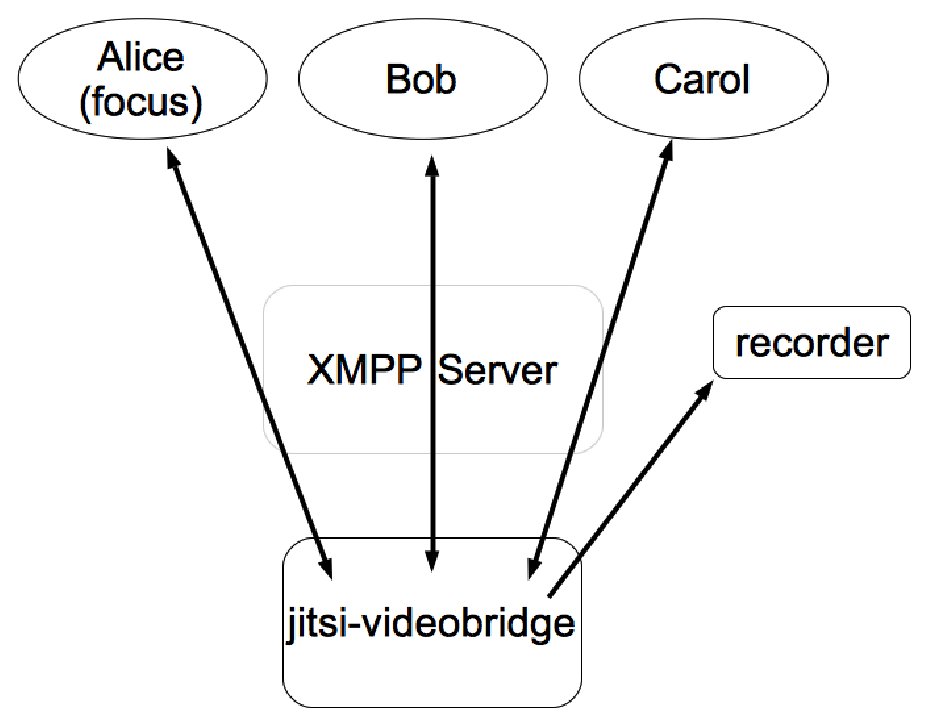
\includegraphics[width=0.4\textwidth]{./pics/jm-rec.eps}
        \caption{A recording application connected to a \jm\ conference as a "fake" participant.}
   \label{jitmeet-rec}
\end{wrapfigure}

Since the participating clients are running an application within their
browser, if we want one of them to do recording, we would need modifications to
the browsers. This is inconvenient because users would need to use modified
browsers, and because in most use-cases the recordings are going to be stored
(and post-processed) on a server, so they would have to be transferred there
somehow.  To avoid this, a "fake" participant can
be added, which does not not actually participate in the conference
(does not send audio or video), and runs on a server (and without the need for a browser at all). Still, it
connects as a normal participant and establishes an RTP session with \jvb\ (see
figure \ref{jitmeet-rec}).


Recording directly on \jvb\ is more straightforward, so our initial
implementation was focused on that. However, most of the code resides in \lj, allowing
it to be easily reused.

Shunyang Li, a student from Peking University, is currently working, under my
guidance and within context of the Google Summer of Code program, on
\emph{Jirecon}\footnote{https://github.com/jitsi/jirecon}-- a standalone XMPP
container for the recording application described here.



\section{Implementing support for the WebRTC transport layer}
The documents from the RTCWEB working group at the IETF specify how multimedia
is to be transported between WebRTC endpoints. In the most part existing
standards are reused.

It is mandatory to use the Interactive Connectivity Establishment (ICE\cite{ice}) protocol to
establish a session. This assures that an endpoint will not send any media
before it has receive consent (in the form of a STUN message) from the remote
side. This protects against possible traffic augmentation attacks, in which a malicious
web-server causes browsers to send large amounts of data (e.g. a video stream) to a
target.

After a connection is established using ICE, a DTLS-SRTP session is started.
This means that the endpoints use Datagram TLS (DTLS\cite{dtls})
to exchange key material, which is then used to generate session keys for a
Secure Real-Time Protocol (SRTP\cite{srtp})
session. The procedure is defined in RFC5763\cite{rfc5763}.
In a \jm\ conference, each participant's browser setups two SRTP sessions with
\jvb\ in this way.

\medskip
SRTP provides an unreliable transport. For this reason \wrtc\ uses a couple of
mechanisms on top of SRTP to improve the quality of the media. These mechanisms
and their implementation in \lj\ are discussed in sections \ref{red} to
\ref{rtx}. Before that section \ref{lj} gives an overview of the RTP stack used
in \lj.


\subsection{The RTP stack in \lj}
\label{lj}

\begin{wrapfigure}{R}{10cm}
    \centering
    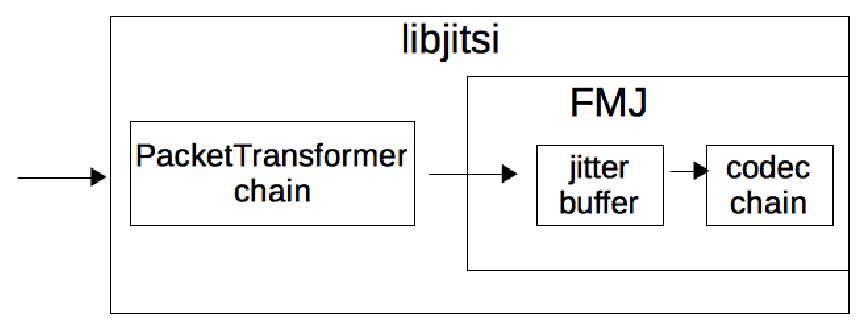
\includegraphics[width=9cm]{./pics/lj.eps}
    \caption{General scheme of the RTP stack in \lj.}
    \label{lj-scheme}
\end{wrapfigure}

\lj\ makes heavy use of the Freedom for Media in Java
(FMJ\footnote{http://sourceforge.net/projects/fmj/}) library. This is an
open-source implementation of the Java Media Framework (JMF) API, and it is
used in \lj\ for a variety of tasks: capture and playback of media, conversion
(transcoding) of media, and for handling of basic RTP streams. FMJ is highly extensible, and
many components (such as media codecs, capture devices and renderers) are written in \lj.


The RTP stack used by FMJ lacks some features: notably support for SRTP and 
for asymmetric payload type mappings (i.e. sending and receiving a given format
with two different RTP payload type numbers). In order for \lj\ to implement these features, it
intercepts the RTP packets from the actual socket in use, and processes them
before passing them on to FMJ. Specifically, packets go through a chain of
\emph{PacketTransformer}s, which perform various tasks. Figure \ref{lj-scheme}
illustrates this scheme.

\begin{wrapfigure}{R}{4cm}
   \centering
        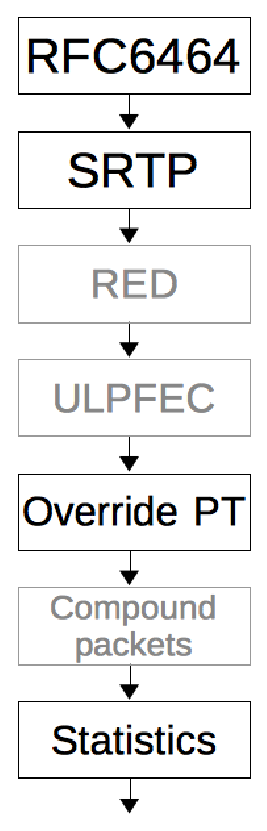
\includegraphics[width=3cm]{./pics/lj-pt.eps}
        \caption{The chain of \emph{PacketTransformer}s in \lj. The shaded elements are new additions.}
   \label{lj-pt}
\end{wrapfigure}
\emph{PacketTransformer}s provide a convenient interface to intercept RTP and
RTCP packets at different stages of their processing and perform additional
operations on them. Despite their name, \emph{PacketTransformer}s don't need to change
the packets in any way, they can be used just for monitoring. 

Figure \ref{lj-pt} lists the currently used \emph{PacketTransformer}s in \lj. A
packet which arrives from the network goes through the chain downwards (and
when packets are sent, they go through the same chain but in the other
direction). The transformer labelled "RFC6464" is used to extract the
audio level information from packets, which include this information in
an RTP header extensions defined in RFC6464\cite{rfc6464}. The audio
levels are used for, among other things, performing dominant speaker
identification (see section \ref{dsd}). This transformer also serves
as a filter, dropping packets with audio marked to contain silence (in order to
avoid unnecessary processing, which is why the transformer is first in the
chain). The SRTP transformer decrypts SRTP packets. The
"Override PT" transformer changes the payload type numbers of packets. It is
used to implement asymmetric payload type mappings. The statistics transformer
monitors RTCP packets and extracts statistics from them, making them available
to other parts of the library.

The rest of the transformers (the ones in grey) were added with the
implementation of the recording system, and will be discussed in the next
sections.




\subsection{RED}
\label{red}
RFC2198\cite{red} defines an RTP payload-type that allows the encapsulation of
one or more "virtual" RTP packets in a single RTP packet. It is intended to be
used with redundancy data. Its use is negotiated as a regular media format and
it does not have a static payload-type number, so a dynamic number is assigned
during negotiation.

In \wrtc, RED is supported and used for video streams. In the case of a \jm\
conference, it is negotiated between the clients, and \jvb\ has no way of
affecting its use or its payload-type number, because it does not actively
participate in the offer/answer procedure. This means that in order to record
video, the recorder has to understand RED.

\smallskip
We decided that the best way to implement RED in \lj\ is as
a \emph{PacketTransformer}. There was one complication--
\emph{PacketTransformer}s work with single packets (they take a single packet
as input and produce a single packet as output), while a RED packet may contain
multiple "virtual" RTP packets which would need to be output.

We modified \lj, so that all \emph{PacketTransformer}s work with multiple
packets at a time-- they take an array of packets as input and produce an array
as output. This change was not easy, because we had to make sure that we didn't
break existing code, but it proved useful later on when we added support for
ULPFEC and RTCP compount packets.

We implemented a RED packet transformer following RFC2198 and inserted it in
the transformer chain, after the SRTP transformer.




\subsection{Uneven Level Protection Forward Error Correction}
\label{ulpfec}
In general, Forward Error Correction (FEC) refers to a mechanism which allows
lost data to be recovered without retransmission. It involves sending redundant
data, in one way or another.

RFC5109\cite{ulpfec} defines a specific RTP payload-type for
redundant data called Uneven Level Protection FEC (ULPFEC). It is generic in
the sense that that it can be used with any media payload-type
(audio or video, no matter what the codec is). 

In \emph{webrtc.org},
ULPFEC is used with video\footnote{For audio, Opus' own FEC scheme which works
differently than ULPFEC is used (and it is already supported in \lj).},
and while not strictly mandatory for our video-recording (as opposed to RED),
it is important because by decreasing the number of irretrievably lost packets,
it will improve the quality of the recordings.

ULPFEC (in the rest of the section we refer to it as simply FEC) is applied to
an RTP stream (the "media stream", with "media packets")
and adds additional packets to it ("FEC packets"). The basic idea is simple --
take a set $S$ of a few media packets and apply a parity operation (XOR) on it,
resulting in a FEC packet $f$. If any one of the packets in $S$ is lost,
the receiver can use the rest of the packets in $S$ together with $f$ to reconstruct the
lost packet\footnote{This is similar to how RAID5 works.}. 

Along with the parity data, a FEC packet contains two fields which are used to
describe the set $S$ from which it was constructed: a "sequence number base"
field, and a bitmap field that describes the sequence numbers of the packets in
$S$ using the base. The packet $f$ is said to "protect" the packets in $S$. This scheme 
allows FEC to work without any additional
signalling (apart from the payload-type number negotiated during session
initialization). 

The amount of FEC packets added to a stream can be controlled by changing the
number of protected packets, and this can be done dynamically by the sender, to
adapt to network conditions. This is the most common way to use FEC, and the
one currently employed by \wrtc: a given fraction of the configured bandwidth
is allocated for FEC, and it is changed depending on the packet loss
statistics received with RTCP. The aim is to mitigate the effects of packet
loss without retransmissions. 

Another way to use FEC is for probing the available bandwidth. When the sender
detects stable network conditions, it wants to increase its sending bitrate, in
order to improve quality. However, this risks causing a congestion, and therefore
packet loss. The sender initially increases its sending rate by significantly
increasing the amount of FEC. In this case, even if a congestion occurs, the receiver
is more likely to be able to reconstruct the media packets (without the need for
retransmissions). The sender then monitors the following RTCP reports. If they
indicate a high percentage of packet loss, the sender goes back to the
previous, lower rate. Otherwise, the sender can keep the total bitrate, but decrease
the rate of FEC, using the available bitrate for the encoder instead, thus improving
the video quality. This scheme is examined in \cite{NagySOE13}.


\paragraph*{Implementation}
We decided to implement FEC as another \emph{PacketTransformer}. This is how it works:

Two buffers of packets are kept: $bMedia$ and $bFEC$. With every FEC packet $f$
is associated the number $numMissing(f)$ of media packets protected by $f$
which have not been received.

On reception of a media packet, the values $numMissing(f)$ are recalculated for
all $f$ in the $bFEC$ buffer. Then, for all $f$ in $bFEC$: if $(numMissing(f)
== 0)$, then $f$ is removed from $bFEC$. If $numMissing(f) > 1$, then do
nothing. If $numMissing(f) == 1$, use $f$ and $bMedia$ to reconstruct a media
packet and remove $f$ from $bFEC$.

On reception of a FEC packet $f$, $numMissing(f)$ is calculated, and the same
as above is done according to its value.

$bFEC$ is limited to a small size and if a new FEC packet arrives while it is
full, the oldest FEC packet is dropped. This prevents "stale" FEC packets (for
which $numMissing$ will always be $>1$, because more than one of their
protected packets have been lost) to accumulate and cause needless computation.


\medskip
RFC5109 does not place any restrictions on the placement of FEC packets within
a stream, and in our architecture FEC packets are handled entirely in the FEC
\emph{PacketTransformer} and not passed on to the rest of the application. This
presents a potential problem for the depacketizer (see section
\ref{depacketizer}), because it cannot differentiate
between a sequence number missing because a packet was lost and a sequence number missing
because it was used by a FEC packet.

For this reason we initially implemented re-writing of the RTP sequence numbers of
the media packets after they pass the \emph{PacketTransformer}-- we decreased their
number by the number of FEC packets already received (see figure \ref{fec-seqs} for an
illustration). This still leaves some problems, because a lost FEC packet might be
incorrectly interpreted as a missing media packet, and because packets might be
incorrectly re-numbered when a packet has arrived out of order.

\begin{figure}[h]
   \centering
        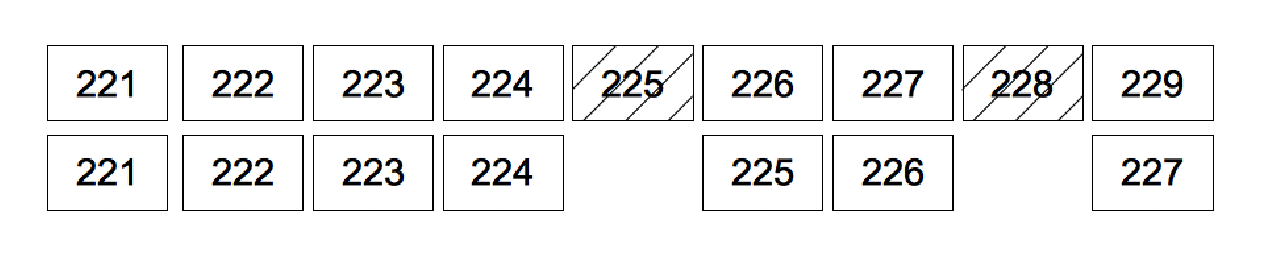
\includegraphics[width=0.9\textwidth]{./pics/fec-seqs.eps}
        \caption{Re-writing sequence numbers after removal of FEC packets. The
        marked packets are FEC. The line above shows the sequence numbers
        before FEC is removed, the line below-- after.}
   \label{fec-seqs}
\end{figure}

Upon further research we found that \wrtc\ restricts the placement of FEC
packets in the stream by only adding them at the end of a VP8 frame, after the
RTP packet with the \emph{M}-bit set (see section \ref{recording-video}). This
restriction allows the depacketizer to distinguish between the case of a lost
part of a frame and a sequence number being used for FEC, and makes re-numbering
of the media packets unnecessary.




\subsection{Retransmissions}
\label{rtx}
RFC4585\cite{rfc4585} defines a type of RTCP Feedback Message (called NACK), with
which a received can indicate to a sender that a specific RTP packet (or a set
of packets) has not been received. Upon receipt of a NACK, a sender might attempt to
retransmit the lost packets. 

In \wrtc\ NACKs and retransmissions are used for
video streams. Current versions do retransmissions by sending the exact same
RTP packets (without even re-encrypting, which causes some SRTP implementations
to falsely detect a replay attack), but there's planned switch to using the
payload format defined in RFC4588\cite{rfc4588} to encapsulate retransmitted packets.

Currently \lj\ does not support RFC4588, but we plan to implement it (as
another \emph{PacketTransformer}). Retransmitted packets are not handled in a
special way-- we just ensure that we have
buffers of sufficient size so that retransmitted packets are not dropped as arriving too late (see section \ref{video-jb}).

\medskip
When the recording application runs on the \jvb, requesting retransmissions with NACKs is not
very important, because all RTP packets go through the bridge, and if the
bridge is missing a packet, then so are the rest of the participants. The recorder can
rely on the participants for sending NACKs, and just make use of the retransmissions themselves.  
However, when the recorder runs in a separate application (as a "fake"
participant), this approach doesn't work, because packets might be lost between
the bridge and the recorder. Our implementation does not yet support sending NACKs, but we plan
to introduce it.




\subsection{RTCP compound packets}
RFC3550 specifies that two or more RTCP packets can be combined into a compound
RTCP packet. The format is very simple -- the packets are just concatenated
together and the length fields in their headers allow their later
reconstruction.

Because of the lack of support for such packets in FMJ (and because \wrtc\
makes use of them), we implemented it in \lj\ (as a \emph{PacketTransformer}).




\section{Recording video}
\label{recording-video}
\subsection{The VP8 codec}
The WebRTC standards do not define a video codec which has to be supported by all clients. There
has been a very long discussion at the IETF
about whether to make a codec mandatory to implement (MTI), and if so, which one. The
four main options suggested were
\emph{(i) make the VP8 codec MTI};
\emph{(ii) make the H264 codec MTI};
\emph{(iii) have no MTI codecs};
\emph{(iv) make both VP8 and H264 MTI}. No consensus has been reached.
Nevertheless, currently VP8 is the de-facto standard codec for WebRTC, because
it is the only codec supported by \wrtc\ (and therefore \jm).


VP8 is a video compression format, defined in RFC6386\cite{vp8}. It was
originally developed by \emph{On2 Technologies}, which was acquired by
\emph{Google} in 2010. \emph{Google} published the specification and released a
reference implementation (\emph{libvpx}) under a BSD-like opensource
license. They also provided a statement granting permission for royalty-free
use of any of their patents used in
\emph{libvpx}\footnote{http://www.webmproject.org/license/additional/}.


Both VP8 in general and \emph{libvpx} work exclusively with the I420 raw
(uncompressed) image format\cite{i420}.
A component called a VP8 encoder, which takes as input an I420 image and produces a "VP8
Compressed Frame". Similarly, a decoder reads VP8 compressed frames and
produces I420 images.

A separate specification\cite{vp8rtp} defines how to transport a VP8 compressed
frame over RTP. In short, the process involves optionally splitting a VP8
compressed in parts, prefixing each part with a structure called a "VP8 Payload
Descriptor", and then encapsulating each part in RTP. This process is referred
to
as packetization, and the reverse process (of collecting RTP packets and
constructing VP8 compressed frames)-- depacketization. Figure \ref{vp8-scheme}
provides a high-level overview of the use of VP8 with RTP.

\begin{figure}[h]
    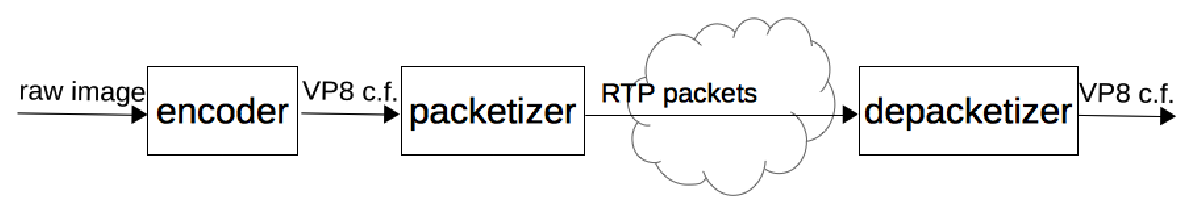
\includegraphics[width=0.9\textwidth]{./pics/vp8.eps}
    \caption{Using VP8 over RTP (c.f. stands for "compressed frame")}
    \label{vp8-scheme}
\end{figure}

\lj\ already has a VP8 implementation, which is used in the \j\ client and
consists of four parts: an encoder and decoder (wrappers around \emph{libvpx}),
a packetizer and a depacketizer. For the purposes of recording, we need 
only a depacketizer. We found that the existing depacketizer is not compliant with
the specification, and also not compatible with \wrtc. We decided to re-write it from scratch.

\subsection{Depacketization}
\label{depacketizer}
The VP8 Payload Descriptor can be thought of as an extension to the RTP header. It has variable length (between 1 and 6 bytes) and contains, among others, the following fields:
\begin{itemize}
\item \emph{S}-bit: start of VP8 partition, set only if the first byte of the payload of the packet is the first byte of a VP8 partition.
\item \emph{PID}: Partition ID, specifies the ID of the VP8 parition to which the first byte of the payload of the packet belongs.
\item \emph{PictureID}: A running index of frames, incremented by 1 for each subsequent VP8 frame.
\end{itemize}

Apart from this, the depacketizer also uses the following fields from the RTP header:
\begin{itemize}
\item \emph{Timestamp}: a 32-bit field specifying a generation timestamp of the payload. For VP8, all RTP packets from a given frame have the same timestamp.
\item \emph{Sequence number}: An index of RTP packets.
\item \emph{M}-bit: set for the last RTP packet of a frame (and only for it).
\end{itemize}

We implemented the algorithm suggested in the specification: we buffer RTP
packets locally, until we receive a packet from a new frame. At this point, we
check whether the buffer contains a full VP8 frame, and if it does we output
it. Otherwise, we drop the buffer and start to collect packets for the next
frame. In \lj, the depacketizer is part of the FMJ codec chain (see fig. \ref{lj-scheme}).

In order to decide whether a received packet is from a new frame or not, the
RTP timestamp and the \emph{PictureID} fields are used (if either don't match,
then it's a new frame). 

The \emph{PID} and \emph{S} fields from the VP8 Payload Descriptor allow us to
detect the first packet from a frame -- the first, and only the first packet
will have both the \emph{S}-bit set and \emph{PID} set to 0.

This allows us to easily check whether we have a full packet
in the buffer or not: we have a full packet if: \emph{(i) we have the beginning
of a frame}; \emph{(ii) we have the end of a frame (a packet with the M-bit
set)}; and \emph{(iii) we have
all RTP sequence numbers inbetween}.

The following pseudo-code outlines the procedure.

\begin{lstlisting}[frame=single]  % Start your code-block
hack
receive(Packet p){
    if (!belongsToBuffer(p))
        flush();
    push(p);

    if (haveFullFrame())
        outputFrame();
}

belongsToBuffer(p){
    if (bufferEmpty())
        return true;
    else if (bufferRtpTimestamp == p.RtpTimestamp 
             && bufferPictureID == p.PictureID)
        return true;
    return false;
}

haveFullFrame(){
    if (! (buffer.first.S && buffer.first.PID == 0))
        return false;
    if (!buffer.last.M)
        return false;
    for (int i=buffer.first.seq; i<=buffer.last.seq; i++)
        if (!buffer.contains(i))
            return false;
    return true;
}
\end{lstlisting}


\subsection{Container format}
After depacketization, we are left with a stream of VP8 Compressed Frames. We needed to decide how to store them on disk. We considered three options:
\begin{itemize}
\item Use the \emph{ivf} container format
\item Define and use our own container format
\item Use the \emph{webm} container format
\end{itemize}

The \emph{ivf} format is a very simple video-only, VP8-only storage format. It
was developed with \emph{libvpx} for the purposes of testing the
implementation. It precedes each frame with a fixed-size header containing just
the length of the frames and a presentation timestamp. The only advantage of
using this format is the relative simplicity of it's implementation. The disadvantages
include that not many players support it (for example browsers don't support it), and
that it's lack of extensibility.

Defining our own container format has one advantage, and that's the possibility
to design it in a way that allows partial VP8 frames. The \emph{libvpx} decoder
has a mode which allows it to decode a frame even if parts of it are missing.
In order to use this API, however, the decoder needs to be provided with
information about which parts (which VP8 partitions) are missing, and this
information would be lost if we use \emph{ivf} or \emph{webm}. The
disadvantages of this approach are the complexity that it brings, and the
inflexibility with regards to the players -- no of the other tools which
we use (like \emph{ffmpeg}) will be able to handle it, and we would need to
implement our own decoder.

The \emph{webm}\cite{webm} format is a subset of
\emph{matroska}\cite{matroska}. It has been designed
specifically to contain VP8 (possibly interleaved with audio) and to be played
in browsers. It allows for much more flexibility than \emph{ivf}. The main advantage
is that it can be played by many players, and that it supports many features,
so we can later extend our implementation if needed.

\smallskip
We found a small library (written in C++, but with Java mappings already
available) with a simple API that would allow us to write \emph{webm} files
easily, so we decided to ignore \emph{ivf}, postpone the potential
definition of a new format, and use \emph{webm}. 

We adapted the library to our needs, and implemented a \emph{WebmDataSink} class which takes
as input a stream of VP8 compressed frames and saves them in a \emph{webm} file.

\medskip
A VP8 stream transported over RTP does not have a strictly defined frame rate.
Each VP8 frame has it's own, independent timestamp, generated by the source (usually at the
time of capture from a camera, before VP8 encoding has taken place), and this timestamp
gets translated into an RTP timestamp and is carried in RTP.

When we save VP8 in \emph{webm} format, we use the RTP timestamp in order to calculate
a presentation timestamp. This is simple-- for the first recorded frame we use
a presentation timestamp of 0 (in milliseconds) and for subsequent frames we
calculate the difference from the first frame.


\subsection{Requesting keyframes}
VP8 has two types of frames: I-frames (or keyframes) which can be decoded
without any other context, and P-frames, whose decoding depends on previously
decoded frames. In order to start working, a VP8 decoder needs to first decode a keyframe.
Therefore, we want the recorded \emph{webm} files to start with a keyframe.

Because keyframes are rarely sent, and because we want to be able to start
recording a conference at any time, we needed a way to trigger the generation of a
keyframe. One way to do this, which is supported by \wrtc, is by the use of
RTCP Full-Intra Request (FIR) feedback messages (defined in
RFC5104\cite{rfc5104}, section 3.5.1).

We added support for FIR messages in \lj\ and made use of them to request
keyframes in the beginning of a recording. We faced a difficulty because FIR
messages contain an "SSRC of packer sender" field, and \wrtc\ clients only
accept messages from SSRCs that they know about (that is, that have been
specifically added via signalling). We had to make \jvb\ generate and use it's
own SSRC, which it also announces to the focus via COLIBRI.

\subsection{Jitter buffer}
\label{video-jb}
A jitter buffer is normally used in a real-time multimedia application to
introduce a certain amount of delay in the playback of media,
mitigating the effects of the varying delay of packets on the network
(the jitter). A buffer which is too small gets emptied quickly when packets are
delayed and playback has
to be paused. A buffer which is too big adds unnecessary delay to the playback.
For this reason adaptive jitter buffers are used, which change their
size according to network conditions.

In the case of video with WebRTC, apart from just jitter on the network, there
might be packet retransmissions triggered by the receiver (which necessarily
arrive at least one RTT later than the originally transmitted packets), and it is beneficial if the
buffer is large enough to accept them (as opposed to dropping them because they
have arrived too late).

For the purposes of recording, a relatively long delay (on the order of a few
seconds) is acceptable, provided that the buffer can be emptied at the end of the recording,
without packets being discarded. For this reason we decided to use a fixed-size
jitter buffer.

FMJ already includes a jitter buffer in its chain (see figure \ref{lj-scheme}), but
for technical reasons it was hard to implement a way to empty it without
discarding its contents. We decided to implement our own buffer, in the form of
a \emph{PacketTransformer}. For simplicity, we limited its size to a given
number of packets, and not to a given length of time. We used a default size
of 300 packets, since we observed that this usually corresponds to between 3
and 10 seconds.

\subsection{An overview of the whole process}
\label{recording-video-overview}
The components discussed above are pieced together in a \lj\ class named \emph{RecorderRtpImpl}\footnote{Because it implements the \emph{Recorder} interface, using RTP as opposed to a capture device as input},
which we implemented specifically for recording video\footnote{Although we
later adapted it to record audio as well.}.

\emph{RecorderRtpImpl} takes its input in the form of RTP
packets. It first demultiplexes the packets by their SSRC, and puts them in a jitter
buffer, which is placed as the last element of the \emph{PacketTransformer} chain in figure \ref{lj-scheme}.

After they exit the jitter buffer, all packets
are passed to an instance of FMJ which is configured to transcode from the
"VP8/RTP" format, to the "VP8" (i.e. to do depacketization). FMJ does it's own
demultiplexing and creates a VP8 depacketizer for each stream. The depacktizer
is part of the FMJ codec chain (again, see figure \ref{lj-scheme}), and the
internal FMJ jitter buffer is practically not used. The output of FMJ is in the
form of a stream of VP8 compressed frames, which is passed to a
\emph{WebmDataSink} instance, which produces the final \emph{webm} file.

As soon as a new VP8 stream is detected, before its packets enter the jitter
buffer, a keyframe is requested, by sending an RTCP FIR message. 

When the recording of a stream is stopped (either because of a user request
via the API, or because an RTCP BYE message is received, or because of a
timeout), the jitter buffer for the specific SSRC is emptied, its contents
being processed.

Using this process, each SSRC stream (with the VP8 format) is saved in a
separate \emph{webm} file.




\section{Recording audio}
\label{recording-audio}
The WebRTC standards define two mandatory to implement audio codecs:
\emph{G711}\cite{g711} and \emph{Opus}\cite{opus}. All WebRTC endpoints are
required to implement them.

\emph{G711} is an audio codec originally developed in the 1970s by the ITU for
use in the telephone network. It works on an input PCM signal with a sampling
rate of 8000Hz (which already limits the sound quality) and produces an encoded
signal with a constant bitrate of 64kbps. It is included in WebRTC for interoperation
with legacy devices.

\subsection{Opus}
\emph{Opus} is a modern audio codec, whose definition was published as an RFC in 2012. It has a variable bitrate
and works with fullband sound (sampled at 48000Hz). The average bitrate is configurable,
and at 32kbps (the default in many applications which encode voice) it produces
sound with remarkable quality.

In a \jm\ conference, since all participants use full-fledged
browsers, \emph{Opus} is always the codec being used.

\emph{Opus} supports frames of different size, but almost all applications (includeing \wrtc) use frames of 20ms. 

\emph{Opus} has a build-in FEC mechanism which works differently than the
RFC5109 mechanism discussed in section \ref{ulpfec}. If enabled for a packet,
it encodes the packet at a lower quality, and attaches this
version to the subsequent packet. This allows a single lost packet to be
recovered (in lower quality), but if two consecutive packets are missing, only
one can be recovered. It also has a Packet Loss Concealment (PLC) function, which
can be used in the absence of a packet to produce a low level of noise in such
a way as to reduce audible crackling.

\lj\ has support for \emph{Opus} and for it's FEC and PLC features.


\subsection{Recording a mix directly ("live" mixing)}
When we started work on recording audio, the most straightforward solution,
given the existing code, was to create a mix on-the-spot (in the recording
application) and record a single file. This was because \lj\ has an advanced
audio mixer component, which is used in the \j\ client and \jvb\  (if it is so
configured) to mix the audio for a conference. The API allows the addition of a
basic RTP stream, and handles all the processing (decoding, resampling, if
needed) automatically (see figure \ref{audio-mixer}). Also, the audio mixer
serves as a capture device, and
can thus be recorded with the existing \lj\ recorder.

\begin{figure}[h]
    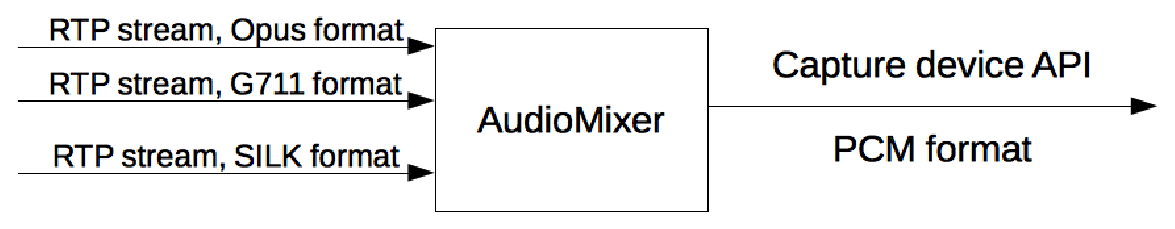
\includegraphics[width=10cm]{./pics/audio-mixer.eps}
    \caption{The API of the \lj\ audio mixer}
    \label{audio-mixer}
\end{figure}

Indeed, the implementation proved easy to do, but we faced a problem when we
started to think about synchronizing the recorded audio and video. In order to
do this, we would at the very least need to know the exact moment where a
stream has been added to the mix. This was very hard to do with the audio mixer
API.

We would also need a way to guarantee that the spacing between two audio
packets in the mix exactly matches the spacing between the packets at the
source. We had no way of doing this with the mixer.

We decided that we needed to give up using the \lj\ audio mixer and
implement code which would allow us finer control over the whole process.


\subsection{Recording streams separately}
Since we were going to implement the code to handle the decoding and recording
of audio streams anew, doing mixing in the application would require additional
work, and would introduce substantial complexity. Additionally, there are already
many tools which allow the mixing of already recorded files. For these reasons, we
decided to record streams individually.

We already had a \emph{RecorderRtpImpl} (see section
\ref{recording-video-overview}) which we used for video, and which performed
many of the things needed for audio as well. We adapted \emph{RecorderRtpImpl}
so that it could handle streams with different formats, including audio
formats.

The existing code in \lj\ supports recording only in
\emph{mp3} format. We decided to use this, for the time being, because it is
relatively easy to transcode it to whatever format is needed in post-processing.

For an audio stream, we use FMJ to decode (to a PCM format), and
then encode it and save it in \emph{mp3} format.



\subsection{Repairing gaps}
In contrast to video in a \emph{webm} file, in which frames have their
individual presentation timestamps, an audio stream consists of just sound
samples to be played one after the other. This means that if some samples are missing
for some reason (e.g. because of a packet lost in the network), the resulting
stream will be shorter than the original. 

When recording a conference, which might last a relatively long time (possibly
hours), the missing samples accumulate, and, when audio and video are merged in
the end, this leads to audio and video drifting apart. In order to solve this
problem, any gaps in the audio streams need to be repaired. 

The \lj\ implementation of \emph{Opus} already repairs gaps on two levels while decoding.
First, it tries to use FEC, which can be used when only a single packet is
missing. Then, in case of 3 or less missing packets, it uses \emph{Opus}' PLC.
But gaps of more than three packets are not repaired.

Apart from lost packets, there is another cause of gaps in the audio streams. When
participants in a conference use the "mute" functionality, their browsers continue to send
audio packets. However, these packets are specifically marked as containing silence using
RFC6464, and \jvb\ drops them. When a participant unmutes, this results in a
gap, which is possibly many minutes long.

Repairing such a gap by adding silence samples would require non-negligible amount
of computation, because all these samples will then need to be encoded. In such cases
it would be better to re-start the
recording for the stream in a new file, giving it its own timestamp in the
metadata, so that it can be properly mixed in post-processing.

To solve this problem, we decided to introduce an element in the FMJ codec chain, which
would be placed between the \emph{Opus} decoder and the \emph{mp3} encoder, and would detect and
handle gaps. We called this the \emph{SilenceEffect}.

It works by monitoring the timestamps of the buffers which pass through it. It
handles small gaps (the length of gaps to consider short is configurable, with
a default of 3 seconds) by inserting the necessary amount of samples (accurate
up to a single sample). For gaps longer than this, it signals to the
\emph{RecorderRtpImpl}, which restarts the recording into a new file.

This scheme allows us to know, for each recorded audio file, the RTP timestamp
of the first RTP packet, the audio from which is contained in the file. This piece of
information allows us to ensure the synchronization of the resulting audio and video files (see
section \ref{synchronization}).


\subsection{Overview}
Initially we started with recording a mix of all audio streams, because that
was the easiest solution. We later changed to recording streams individually.
Each incoming audio stream (which is usually \emph{Opus}, but any of the codecs
supported in \lj\ can be used as well), is first decoded (and re-sampled to
48000Hz, if necessary), then gaps are repaired by inserting silence. Then the
stream is encoded and saved in an \emph{mp3} file. See figure \ref{audio-rec}
for an illustration. If a gaps of more than 3 seconds is detected, we start
recording in a new file.

\begin{figure}[h]
    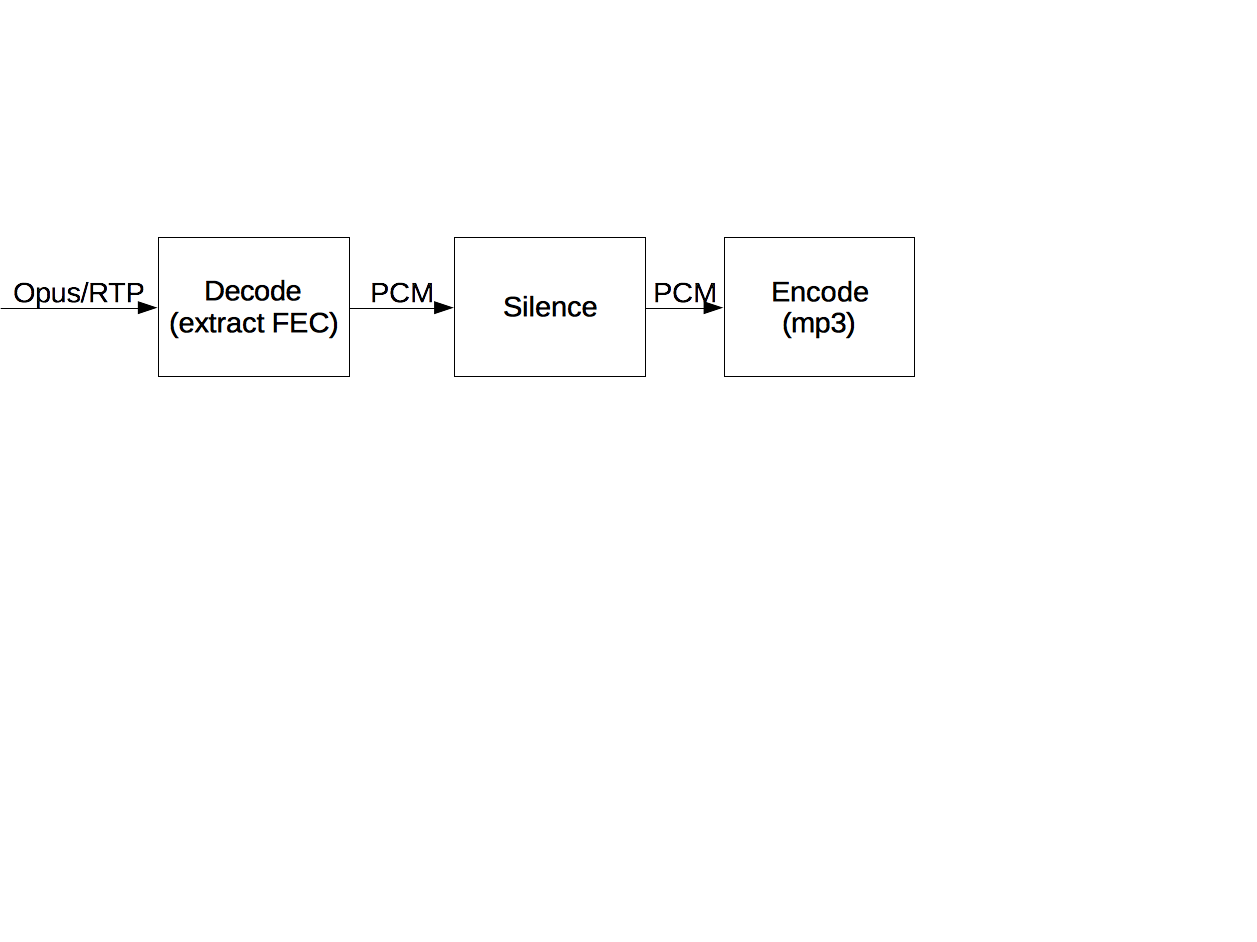
\includegraphics[width=10cm]{./pics/audio-rec.eps}
    \caption{The chain used to transencode audio for the purposes of recording.}
    \label{audio-rec}
\end{figure}

This solution involves re-encoding and that makes it suboptimal -- it is 
more computationally expensive than necessary and reduces the sound quality of the recording.
A better solution would be, whenever possible, to record in a container format
that does can accommodate the original format, and thus does not require
transcoding or even decoding (as we do for video). For \emph{Opus}, a viable
solution would be to use the ogg/opus format and we plan to implement it , see
section \ref{ogg-opus}.






\section{Recording metadata}
\label{recording-metadata}
In order for the post-processing application to correctly process the recorded
audio and video files, it needs some additional information-- a list of file
names, at the very least. In the context of our recording system, we call this information
metadata.

We decided to keep all metadata in a single file, and to use a JSON
format to store it. This would allow to easily extend it with new fields if
the need arises.

We defined a JSON object, which we call a \emph{RecorderEvent}, and the
metadata file consist of two arrays of such objects: one array for audio and
one for video.

All \emph{RecorderEvent}s have two mandatory fields: an event type, and an
instant. The instant is an integer that represents the time at which the event
took place, in milliseconds. No specific clock is used: only the relative time between
the events in a single metadata file is taken into account. There are three types of events:

%\begin{itemize}
%\item RECORDING\_STARTED
%\item RECORDING\_ENDED
%\item SPEAKER\_CHANGED
%\end{itemize}


\smallskip
RECORDING\_STARTED events signify that a recording began in a specific file
(given by the "filename" field), at a specific time. They also contain an "ssrc" field, giving the
SSRC associated with the recording. This field is used by the post-processing
application to associate different files with a single participant, and is
necessary in case recording of a stream is split among more than one file.
These events also contain a "mediaType" field used to distinguish between audio and
video, and two optional fields for additional information about the
participant: "participantName" and "participantDescription". This is used in
post-processing to overlay some text identifying the participant on top of
their video.

\smallskip
RECORDING\_ENDED events indicate that a particular recording ends at a specific
time. These events have "filename", "ssrc" and "mediaType" fields with the same meaning
as for RECORDING\_STARTED events. The post-processing application uses these
events to decide when to remove a certain audio or video stream from the final mix, but they
are optional, because it can determine this from the actual media file.

\smallskip
SPEAKER\_CHANGED events are used to signal that the dominant speaker in the
conference has changed (at a specific time). They include an "audioSsrc" field which specifies the
SSRC of the audio stream of the new dominant speaker, and an "ssrc" field which specifies the SSRC of the
video stream associated with the new dominant speaker. The post-processing application uses SPEAKER\_CHANGED
events to change the video shown in full size.

A few examples of \emph{RecorderEvent}s follow, and appendix
\ref{appendix-metadata} has the full contents of a metadata file from an
actual recording of a conference.

\begin{verbatim}
{
"instant" : 1395767658389,
"type" : "RECORDING_STARTED",
"filename" : "3360910907.webm",
"ssrc" : 3360910907,
"mediaType" : "video",
"aspectRatio" : "16_9",
"participantName" : "Jane Doe",
"participantDescription" : "
}

{
"instant" : 1395767704521,
"type" : "RECORDING_ENDED",
"filename" : "1277672956-2.mp3",
"ssrc" : 1277672956,
"mediaType" : "audio"
}

{
"instant" : 1395767658527,
"type" : "SPEAKER_CHANGED",
"ssrc" : 500778727,
"audioSsrc" : 1277672956
}
\end{verbatim}

\section{Synchronization}
\label{synchronization}
--how is audio synchronized
--how is video synchronize

--how to time them...
Purpose: audio and video from a single participant need to be perfectly synchronized. Need to use the timestamps from the source, because of network jitter. 

How it works: RTCP sender reports and the info they contain.

Can use CNAME, but chrome has a bug (link). We use "endpoint" identifiers obtained from signalling instead.


\subsection{Implementation}
The mappings that we have saved for each SSRC and each endpoint are illustrated
on figure \ref{diagram-sync}. Given the previously saved values for $rtp0,
ntp0, ntp1$ and $local1$, and given the RTP timestamp $rtpX$ for SSRC A, we calculate the local
time $localX$ which corresponds to $rtpX$:
$$localX = local1 + (ntpX - ntp1)$$ 
where $ntpX$ is the source's wallclock time corresponding to $rtpX$, for which we have
$$ntpX = ntp0 + (rtpX - rtp0)$$
Simplifying: $$localX = local1 + (ntp0 - ntp1) + (rtpX - rtp0)$$
Of course we have to take into account the different formats of the timestamps.

\begin{figure}[h]
    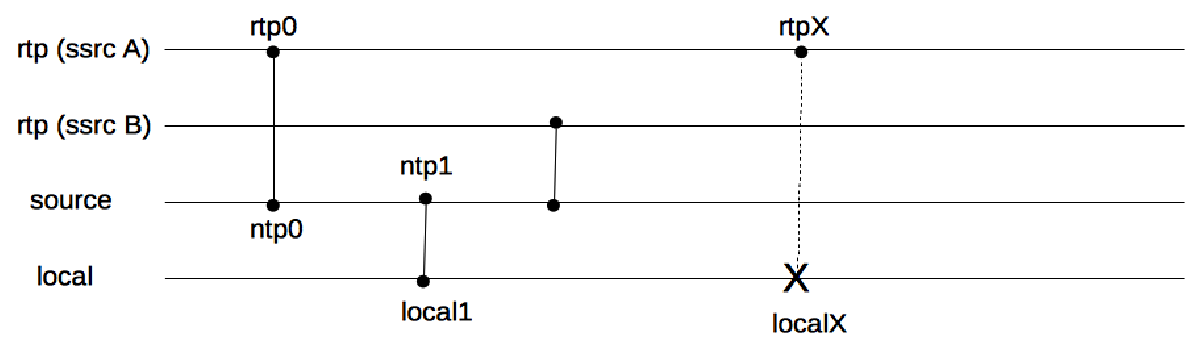
\includegraphics[width=0.9\textwidth]{./pics/diagram-sync.eps}
    \caption{The mappings XXX}
    \label{diagram-sync}
\end{figure}





\section{Dominant speaker identification}
\label{dsd}
Dominant speaker identification (DSI) refers to the process of continuously analysing a set of audio streams
(which are assumed to contain human voice) and keeping track of the one which
comes from the person currently speaking (or the person currently speaking "the
most"). Obviously the problem does not have a single solution, and so it is hard
to measure objectively how well a system performs. A good description of the
general problem and a proposed solution is available in \cite{volfin2012}. 

In a \jm\ conference there are two use-cases for DSI: for "live" use in a
conference and for recording. 
For "live" use, the purpose is to have the client interface change during a
conference, according to who is the dominant speaker (i.e. the video shown in
full changes, following the dominant speaker). In this case DSI is performed
on \jvb, which uses WebRTC data channels\footnote{These are channels which
carry application data (and not audio or video), but are negotiated and
established in the same way as the media channels.}
to notify the clients of the change.

For use in recording, the purpose is for the post-processing application to
take into account the dominant speaker when combining the videos (in general,
it follows the \jm\ interface and renders the dominant speaker in full size).
In this case, DSI is performed by the recording application\footnote{Although,
if the recording application is running as a participant, it can potentially
also open a WebRTC data channel to the \jvb\ and use the events received there,
instead of doing DSI itself.}, and changes of
the dominant speaker are saved as metadata.

\paragraph*{Implementation}
Our first task was to design and implement an API and a simple, non-optimized
algorithm, which we could later improve upon. 

We came up with a very simplified scheme, implemented it and tweaked its parameters until it seemed to
work well in a conversation with two people. It only takes into account the
audio levels (that is, the loudness of the sound) of the different streams. It
works like this:

At all times one stream is considered active, while the rest are considered
'competing'. All streams have an associated score. When new audio levels are
measured for a stream its score is recomputed,
and the scores of all streams are examined in order to determine if one of
the competing streams should replace the then active stream.

In order to be 'eligible' to replace the active stream, a competing stream has to:
\begin{enumerate}
    \item Have a score at least $C$ times as much as the score of the currently active stream.
    \item Have score at least MIN\_SCORE.
    \item Have been active in the last MIN\_ACTIVE milliseconds.
\end{enumerate}

The first rule helps to avoid often changing the active when there are two
streams with similar levels. The second prevents the active speaker from being
changed during a pause of his speech, while no one else is speaking either (but
someone else generates higher levels during "silence" than the speaker). The
third is to make sure that when participants leave a conference, they aren't
mistakenly chosen as active (this is due to implementation details)

The values for the parameters are very dependent on the exact rules for scoring.
We chose the values based on a few uncontrolled experiments we performed. We used
MIN\_ACTIVE $= 1000$ and $C = 1.15$ (MIN\_SCORE is too arbitrary to deserve mention).

Scores are computed as follows: $C_{recent} * avg(0, N_1) + C_{older} * avg(N_1, N_2)$
where $avg(X_1, X_2)$ is the average audio level for the interval $[now-X_2,
now-X_1)$ (in milliseconds). 

Currently the values of the parameters are: $C_{recent} = 2, C_{older} = 1, N_1 = 250, N_2 = 1250$.


\bigskip
We found that this solution works sufficiently well, at least for the purposes
of testing recording and post-processing. One problem that we face is when
one of the participants is generating constant noise (caused for example by a
spinning fan near the microphone). In this case the algorithm tends to select this participant,
even if they are not speaking. One suggestion for a fix is to measure the
variance of the sound levels for a participant, and penalize the score if the
variance is low. This depends on the assumption that a person speaking would
produce sound with varying loudness (and that this variation can be detected
with the 20ms resolution that we use). However, we have not yet tried to solve
this problem.

Lyubomir Marinov has now taken over this task, and has implemented an improved algorithm that more closely resembles the
one proposed in \cite{volfin2012}. However, his implementation still relies on
"audio levels" and not on other analysis of the audio samples. This offers a significant advantage
in our use case, because this information (the "audio level" for a particular RTP packet) is already
calculated by the sending client, and is included in the RTP packet in the format specified in RFC6464\cite{rfc6464}.
This allows \jvb\ to do DSI very cheaply, without the need to decode the received audio streams.



\section{Conclusion}
\label{conclusion}
XXX Crap, I almost forgot about this! Crap!

During the last 6 m we have succ managed to impl a viable recording solution optimal quality and scalability characteristichs. We have also learned the shortcoming of some of our initial ideas, such as live audio mixing and post-processing.

Gathered valuale experience

- de ce que ca a apporte a l’entreprise (realisation)
- de ce que ca vous a apporte (acquisition de competences)

\section{future work}
\label{future-work}
RTX with 4588

requesting RTX with NACK

recording in ogg/opus

\subsection{Recording audio directly in ogg/opus format}
\label{ogg-opus}
postprocessing




\clearpage
\appendix
\section{Jipopro}
\label{jipopro}
\emph{Jipopro} (short for Jitsi Post-Processing) is an application which was created
specifically for post-processing recordings for \jm. It was developed in parallel with
the recording implementation discussed in this document, and is closely tied
with the formats for media and metadata produced by that system. \emph{Jipopro}
is written in Java, but uses external applications for many of its tasks. It's
main author is Vladimir Marinov.

On a very high level, \emph{jipopro} does four things:
\begin{enumerate}
\item Reads a metadata file.
\item Process video producing a single file.
\item Process audio producing a single file.
\item Merges the audio and video files together.
\end{enumerate}

The audio and video processing are independent and could be done in parallel
(but are not, because the audio processing takes a negligible amount of time).


\subsection{Video}
For all video handling, \emph{jipopro} uses \emph{ffmpeg}\footnote{https://ffmpeg.org}.

First every input \emph{webm} file is transcoded to an MJPEG file with a static
frame rate (25fps by default). Then, a timeline of events is constructed
according to the metadata. The events divide the timeline into sections.

For each section, a list of participants, one of whom is active, is maintained.
The sections are then processed (in parallel): a given length of video is taken
(with a specific offset) from the MJPEG file for every participant, and the
obtained video are merged together and saved in an MJPEG file for the section.

After all sections have been processed, they are concatenated together, resulting in
a single MJPEG file.

Then the file is transcoded to a \emph{webm} file.


\subsection{Audio}
For audio handing we use \emph{sox}\footnote{http://sox.sourceforge.net/sox.html}.
First all \emph{mp3} files are converted to \emph{wav} format and padded, if
necessary. All the resulting files are mixed together in a single \emph{wav}
file.

\begin{figure}[h]
    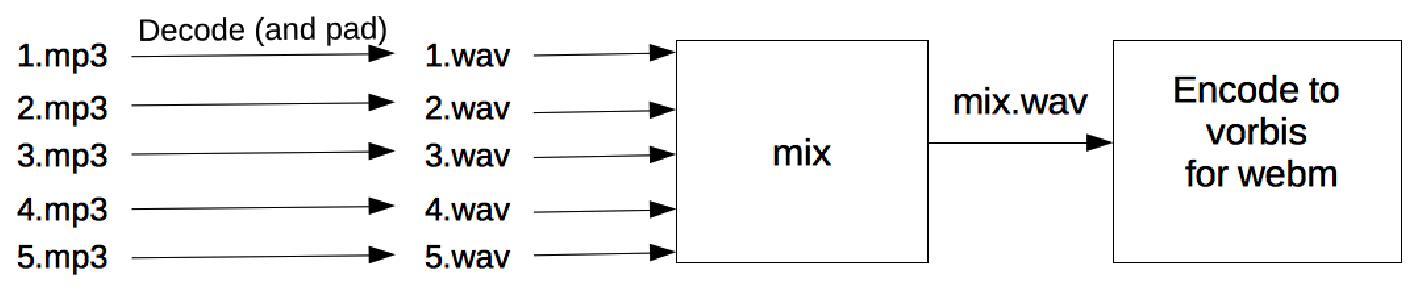
\includegraphics[width=10cm]{./pics/audio-popro.eps}
    \caption{XXX}
\end{figure}


\subsection{Merging}
The resulting audio (a single \emph{wav} file) and video (a single \emph{webm} file)
are combined using \emph{ffmpeg}. The audio is automatically transcoded to \emph{vorbis}, because it is the codec supported by \emph{webm}\footnote{Although the specification is being extended to allow for Opus}.

\subsection{Performance}
performance


\subsection{Future work}
future





\section{The full contents of a metadata file}
\label{appendix-metadata}
\begin{verbatim}
{
  "audio" : [
    { "ssrc" : 2473760775,
      "filename" : "2473760775.mp3",
      "type" : "RECORDING_STARTED",
      "instant" : 1401807483964,
      "mediaType" : "audio" },
    { "ssrc" : 2452647913,
      "filename" : "2452647913.mp3",
      "type" : "RECORDING_STARTED",
      "instant" : 1401807484421,
      "mediaType" : "audio" },
    { "ssrc" : 1107392327,
      "filename" : "1107392327.mp3",
      "type" : "RECORDING_STARTED",
      "instant" : 1401807501709,
      "mediaType" : "audio" },
    { "ssrc" : 1565260729,
      "filename" : "1565260729.mp3",
      "type" : "RECORDING_STARTED",
      "instant" : 1401807524062,
      "mediaType" : "audio"},
    { "ssrc" : 1107392327,
      "filename" : "1107392327-1.mp3",
      "type" : "RECORDING_STARTED",
      "instant" : 1401807527409,
      "mediaType" : "audio"},
    { "ssrc" : 2452647913,
      "filename" : "2452647913-1.mp3",
      "type" : "RECORDING_STARTED",
      "instant" : 1401807532821,
      "mediaType" : "audio"}
  ],

  "video" : [
    { "ssrc" : 2612617218,
      "filename" : "2612617218.webm",
      "aspectRatio" : "16_9",
      "type" : "RECORDING_STARTED",
      "instant" : 1401807484011,
      "mediaType" : "video"},
      
    { "ssrc" : 9413050,
      "filename" : "9413050.webm",
      "aspectRatio" : "16_9",
      "type" : "RECORDING_STARTED",
      "instant" : 1401807484013,
      "mediaType" : "video"},
      
    { "ssrc" : 2612617218,
      "audioSsrc" : 2473760775,
      "type" : "SPEAKER_CHANGED",
      "instant" : 1401807484078,
      "mediaType" : "video"},
      
    { "ssrc" : 9413050,
      "audioSsrc" : 2452647913,
      "type" : "SPEAKER_CHANGED",
      "instant" : 1401807485275,
      "mediaType" : "video"},
      
    { "ssrc" : 1190123626,
      "filename" : "1190123626.webm",
      "aspectRatio" : "16_9",
      "type" : "RECORDING_STARTED",
      "instant" : 1401807500796,
      "mediaType" : "video"},
      
    { "ssrc" : 2612617218,
      "audioSsrc" : 2473760775,
      "type" : "SPEAKER_CHANGED",
      "instant" : 1401807503515,
      "mediaType" : "video"},
      
    { "ssrc" : 2612617218,
      "filename" : "2612617218.webm",
      "type" : "RECORDING_ENDED",
      "instant" : 1401807509187,
      "mediaType" : "video"},
      
    { "ssrc" : 9413050,
      "audioSsrc" : 2452647913,
      "type" : "SPEAKER_CHANGED",
      "instant" : 1401807512310,
      "mediaType" : "video"},
      
    { "ssrc" : 3879530045,
      "filename" : "3879530045.webm",
      "aspectRatio" : "16_9",
      "type" : "RECORDING_STARTED",
      "instant" : 1401807522745,
      "mediaType" : "video"},
      
    { "ssrc" : 3879530045,
      "audioSsrc" : 1565260729,
      "type" : "SPEAKER_CHANGED",
      "instant" : 1401807524818,
      "mediaType" : "video"},
      
    { "ssrc" : 1190123626,
      "filename" : "1190123626.webm",
      "type" : "RECORDING_ENDED",
      "instant" : 1401807534861,
      "mediaType" : "video"},
  ]
}
\end{verbatim}




\clearpage
\bibliographystyle{plain}
\bibliography{bibliography}




\end{document}

XXX: Relaying audio consumes more bandwidth, but is less computationally intensive for \jvb.

%difficulties
\paragraph*{Audio streams}
For audio streams we decided to do the mixing in the application (as opposed to
saving each stream to a separate file and mixing them later). This is because
\lj\ already has all the necessary components. 


\section{Conclusion}
During the internship so far, I have studied in detail how the media transport layers in
a \jm\ conference work, and have implemented support for some of the protocols in \lj. I have also
helped with the design and implemented significant parts of a system which allows the recording of the
audio and video in a \jm\ conference.

During the rest of the internship I hope to improve the existing code and to study in more depth
the problem of dominant speaker detection.

\end{document}

